

\chapter{The state of the Art}
Develop a robot capable of performing a smooth human-like handshake is still a highly interested topic in the scientific literature.
A natural handshake between two humans is a very complex task to replicate, this work just focuses on the interaction force between an artificial hand and a human hand.
The consensus is a complex task to encode inside a robot, participants will easily distinguish the event with respect to another human or to a robot. A human will take into consideration the skin feedbacks like: the temperature, the humidity and the softness. These are some characteristics that are still not embedded into the hardware available in the market. The aspect taken in consideration in this work is the grasping force exchanged in the handshake. 
Robots, nowadays, are highly involved in industries where mostly they have to execute repetitive tasks. These kind of robots, when have to grasp objects, commonly uses multi purposes grippers \cite{multipurposegripper}, therefore, an accurate choice has been done on the hardware to use in this work. 
%The grasping force exchanged in the human-robot handshake event is a complex value to identify, this work is estimating the grasping force from values which can be clearly identified. 


\cite{facialexpressions}
\cite{mirrorgame}
\cite{papageorgiou}

\section{The Idea}
The idea is to create a closed loop controller for the human-robot handshake event, using Pisa/IIT SoftHand produced for research purposes at Universit\`a degli studi di Pisa and Istituto Italiano di Tecnologia (IIT) and upgrading it with four independent FSR sensors which uses an Arduino uno in order to communicate the data.
The FSR sensors are located on the robotic hand so there are no wearing device on the human hand during the execution of the experiments.
This choice leads the work to be focused on the theoretical part of the handshake event, and potentially reach robust results. We are focusing on a general human-robot handshake, knowing that the interaction can vary with participants, f.i. the participant's hand size is affecting the firsts contact points or nominal strength to apply in the handshake can be affected by prior expectations. It is more meaningful then, to study individual differences once the generic case has been studied.
The chosen robotic hand (Pisa/IIT SoftHand) has 19 degrees of freedom and its main characteristic a single dc motor that is pulling a tendon which is embedded in each finger. This physical approach results in an under actuated robotic hand which can be controlled only by the dc motor and can easily adapt to different configurations without modifying the reference position. 

\chapter{Hardware setup}
The hardware must be physically merged in order to reach the goal of a closed loop controller for a handshake. From early approaches as \cite{espen}, an estimation of the human palm has been used.  The \textit{sensorized palm} idea was to approximate the human palm which is the part of the hand mostly interested during a handshake.
The figure \ref{fig:sensorsONhand} shows the position in which the sensors are placed, in particular the n. 1, 2, 3 are placed according studies in \cite{espen}, the sensor n. 4 is placed in order to increase the weight of human-thumb force applied during the grasp.\\ \\

\begin{figure}[h]
  \centering
  \begin{minipage}[b]{0.4\textwidth}
    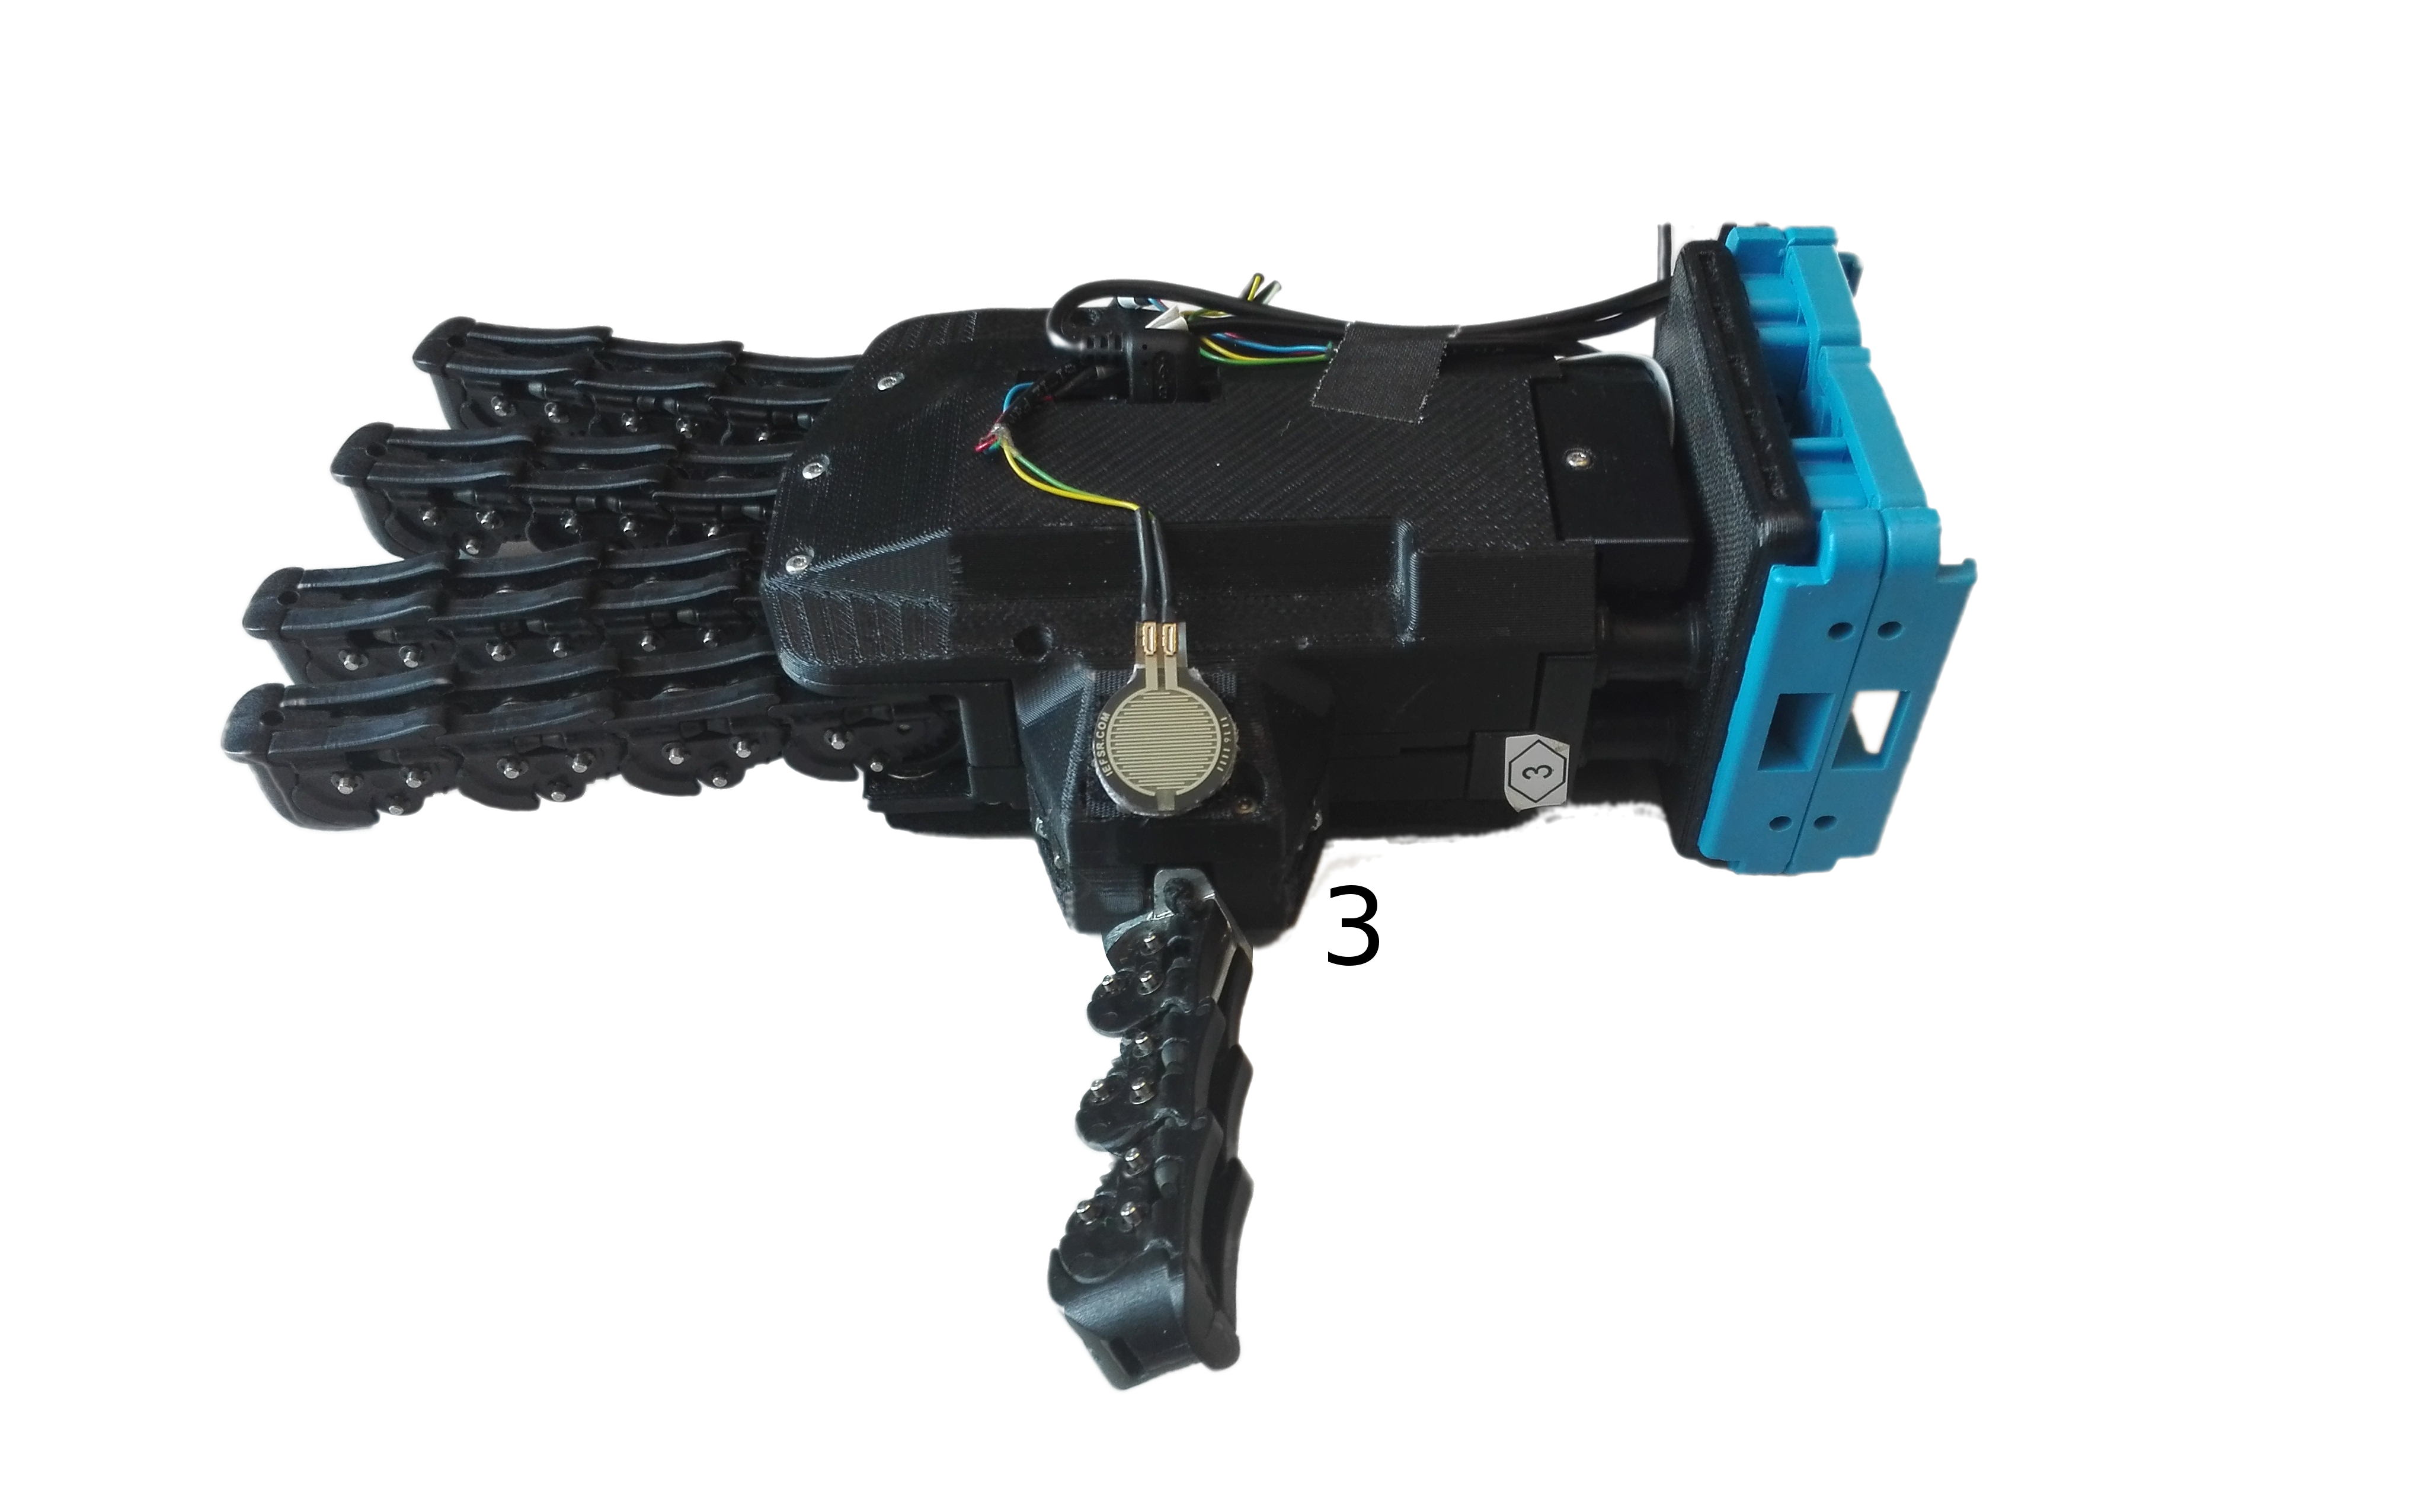
\includegraphics[width=\textwidth]{Figure/qbhand1.png}
    
  \end{minipage}
  \hfill
  \begin{minipage}[b]{0.4\textwidth}
    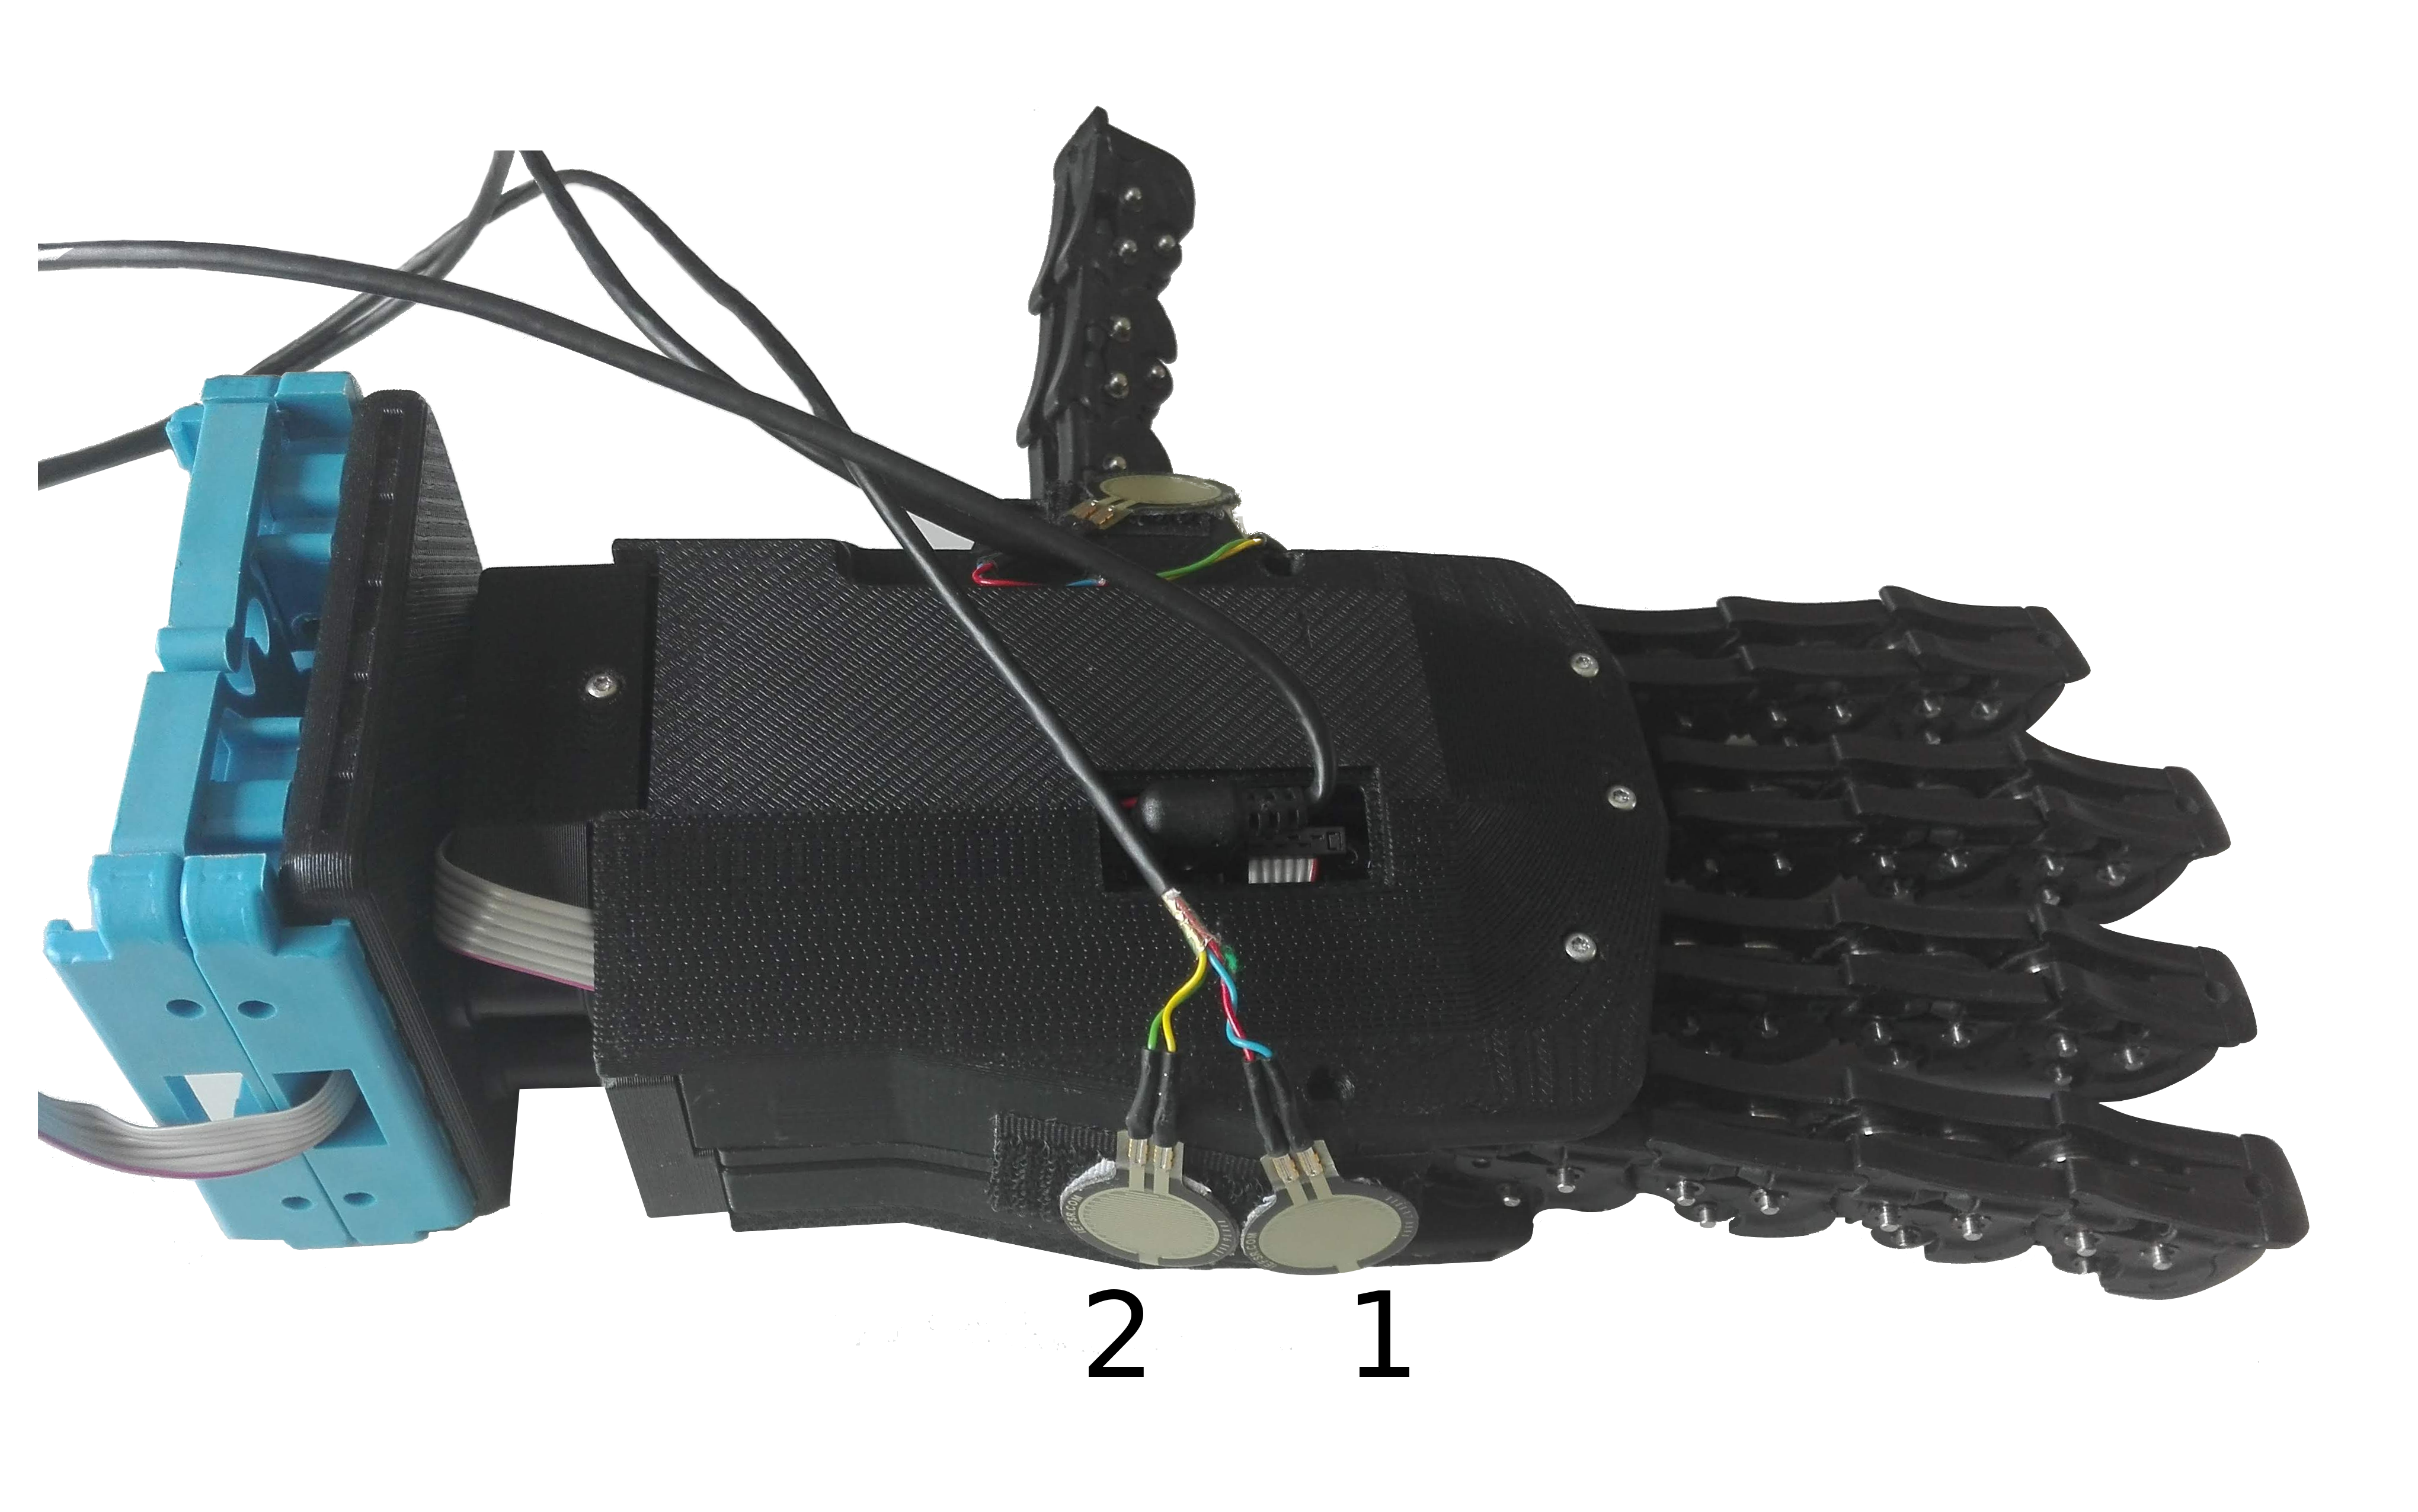
\includegraphics[width=\textwidth]{Figure/qbhand2.png}
  \end{minipage}
  \label{fig:sensorsONhand}
  \caption{Pisa/IIT SoftHand with FSR sensors for handshake}
\end{figure}

\section{The Pisa/IIT SoftHand}
The Pisa/IIT SoftHand is a simple, robust and effective hand designed for grasping and soft manipulation presented in \cite{catalanopisa}. A tick range is provided with the device in order to set a range of possible closure positions, more formally, let's define $q \in \mathbb{N}$ as the closure position of the hand such that $max(q) = 19000$ (Pisa/IIT SoftHand fully closed) and $min(q)=0$ (Pisa/IIT SoftHand fully opened). The hardware is provided with a controller developed by the same group which implements a proportional controller Fig. \ref{Fig:Pr} on the motor position. This enables the researchers to control the Pisa/IIT SoftHand with a reference position, without dealing with the current control of the motor. \\
\begin{figure}[h]
\centering
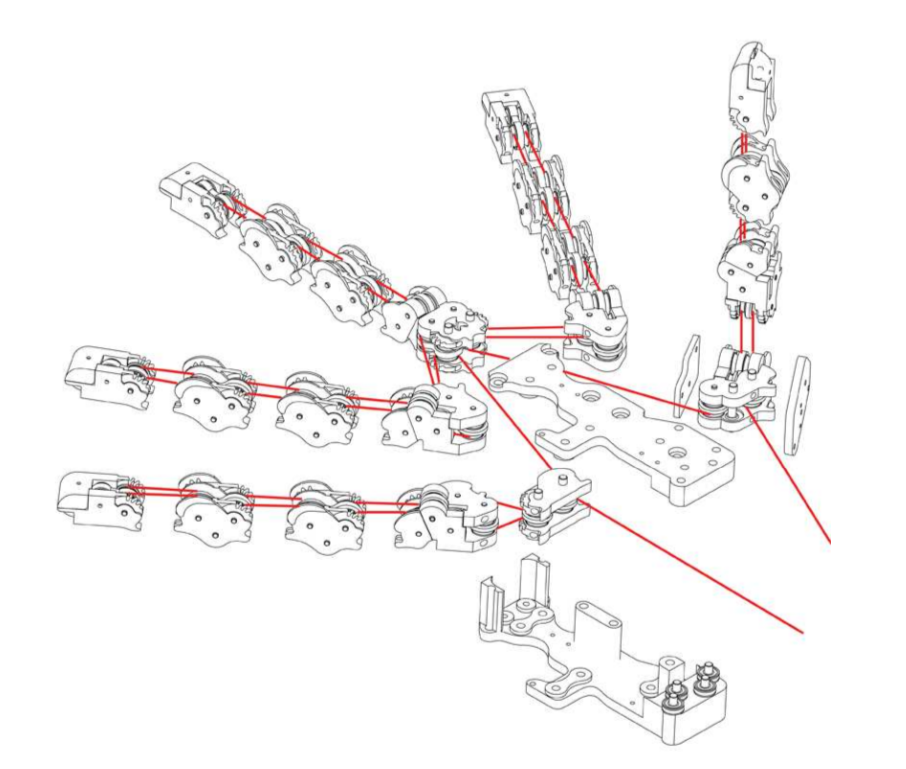
\includegraphics[width=0.6\textwidth]{Figure/softhand.png}
\caption{Exploited view of the modules of Pisa/IIT SoftHand}
\label{Fig:Softhand}
\end{figure}
The proportional coefficient can be set up as preferred since its encoded in ROS as a \textit{rosparam}, this parameter is thought to range between 0 and 1.0. Setting the parameter to 1.0 is minimizing the error value $e(t)$  between the setpoint $r(t)$ and the output $y(t)$.
The successful idea in the design of Pisa/IIT SoftHand can be found in the flexibility of the joints and the wide range of usage.
The reference position $r(t)$ has no 1:1 correspondence with the single physical position of each finger. Having a single motor to control makes the robotic hand really easy to control but introduce uncertainty on the position of each finger. A tendon is running through all the fingers and is pulled by the internal dc motor, therefore a useful available information is the overall tick-position of the Pisa/IIT SoftHand. 
This device has an internal value returning to the system the real tick position, this value is compared with the referenced one in the controller. The real tick position is a value that must be calibrated manually using administrative tools provided by the manufacturers. The calibration is manual which means that the Pisa/IIT SoftHand is manipulated to be into a fully open position and the program save that position as the zero tick position.
%The controller used $C(s)$ is a simple constant controller with value ranges from 0 to 1. 

\begin{figure}[h]
\centering
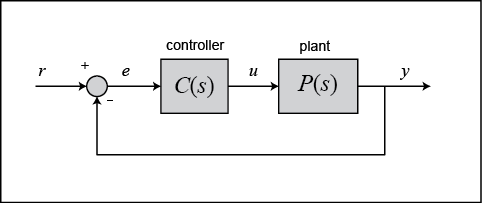
\includegraphics[width=0.5\textwidth]{Figure/feedbackP.png}
\caption{Block Diagram Proportional controller in a feedback loop}
\label{Fig:Pr}
\end{figure}


\section{The Sensors}
The core of the closed loop control is to have a feedback in the whole system which is proportional to the force applied during the handshake from the human. 
\begin{wrapfigure}{R}{0.3\textwidth}
\centering
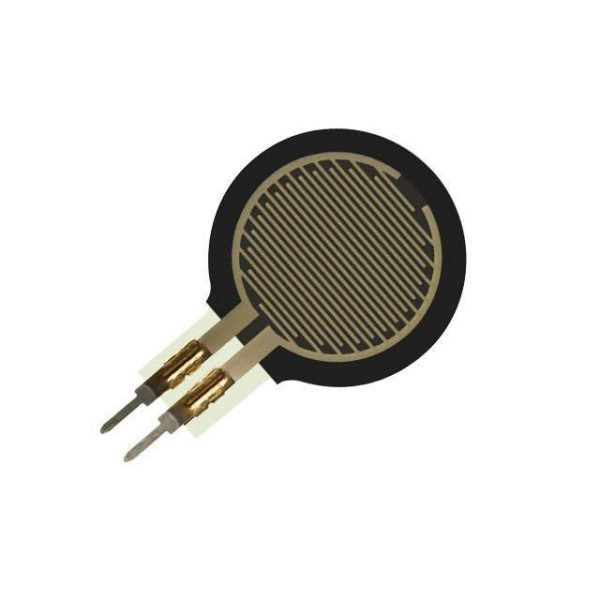
\includegraphics[width=0.25\textwidth]{Figure/fsrsingle1.jpg}
\caption{FSR 13mm}
\label{Fig:FSRsingle}
\end{wrapfigure}

The sensors used in this work are Force Sensitive Resistors Fig. \ref{Fig:FSRsingle} measuring the force applied from the human to the Pisa/IIT SoftHand, in order to decouple this force from the one applied from the Pisa/IIT SoftHand to the human hand, \cite{espen} has been used and the physical position of the FSRs has been setted up accordingly.
FSR sensors are devices that allow to measure static and/or dynamic forces applied on the sensing area, through the variation of its electric resistance. The main advantage of these devices is the low cost per-unit, little space required for installation (thickness under 1.25mm) and the force sensitivity range up to 20N.\\
As robust polymer thick film devices, the FSRs, exhibit a decrease in electric resistance with increase in force applied to the surface. By theory is considered that when a force is applied the resistance changes approximately linear in a logarithmic plot \cite{fsrdatasheet}.
A simple force to voltage conversion is physically implemented as suggested the manifacturer, in fig. \ref{Fig:FSRcircuit} is shown a snippet of the above cited data sheet. For this work \textit{RM} is fixed to $3.3 k \Omega $. 
\begin{figure}[ht]
\centering
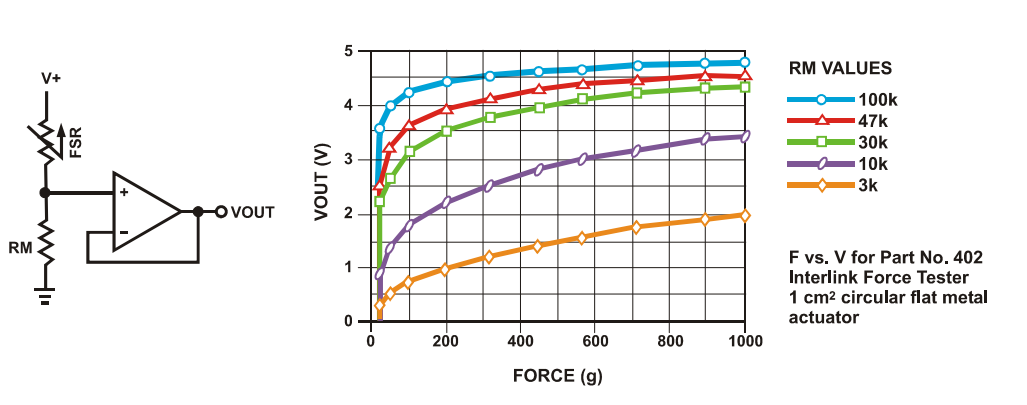
\includegraphics[width=0.7\textwidth]{Figure/fsr.png}
\caption{FSR Datasheet snippet}
\label{Fig:FSRcircuit}
\end{figure}
These mentioned sensors are the more natural choice for handshake experiments since their thickness keeps the size of the Pisa/IIT SoftHand reasonable for human-robot handshake.
% 
Ideally using more sensors allow to get more relevant data but the surface available on the Pisa/IIT SoftHand is limited. The choice in the number of FSR sensors comes from the trade off between using lots of FSR sensors but with a smaller area and using a smaller amount of sensors but with higher area. The first configuration does not ensure the contact among experiments with different participants and the second configuration leads to physical bending of the sensors and influences the consistency of the readings.

 %A calibration method must be used in order to have robust results.

\subsection{Calibration of FSRs}
The calibration procedure of a sensor is a really important task, since it allow to compare experiments and to provide consistent results. 
The first voltage-to-force relation for the FSRs comes from a manufacturer sketch which is returning force with measures standard of grams.
As shown in \cite{calibFSR}, load cells can be used as 'ground truth' to calibrate force sensitive resistors to provide informations in Newtons. 
Using a \textit{sensorized palm} developed in \cite{espen}, sketched in Fig. \ref{fig:dummi} which embeds a load cell and placing the FSR sensors accordingly with the main direction of the force on this \textit{sensorized palm}; values from FSRs and the load cell are compared.\\
Mathematical regression tools have been used in order to find a model that explain the values from the sensors compared to the force of the load cell.
Although an exact calibration of FSR sensors is not the target of this work, a first order model has been fitted to the data in the force-range of interest of this work.
The number of FSR sensors involved in the calibration experiment is two, instead the amount of FSR sensors chosen for the human-robot handshake is four. 
The configuration for the calibration experiment, with the \textit{sensorized palm} and two FRS sensors is shown in Fig. \ref{fig:dummifsr}. In order not to add complexity to this task, is assumed that using two FSR are sufficient to fit a model to the FSR sensors involved in the handshake environment.\\

\begin{figure}[h]
  \centering
  \begin{minipage}[b]{0.4\textwidth}
    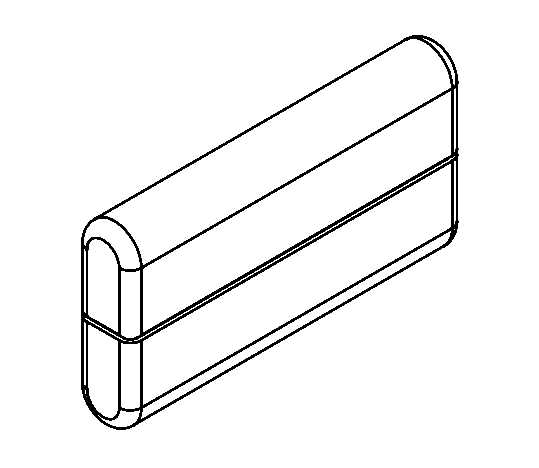
\includegraphics[width=\textwidth]{Figure/dummipalm.png}
    \caption{Sensorized palm}
  \label{fig:dummi}
  \end{minipage}
  \hfill
  \begin{minipage}[b]{0.4\textwidth}
    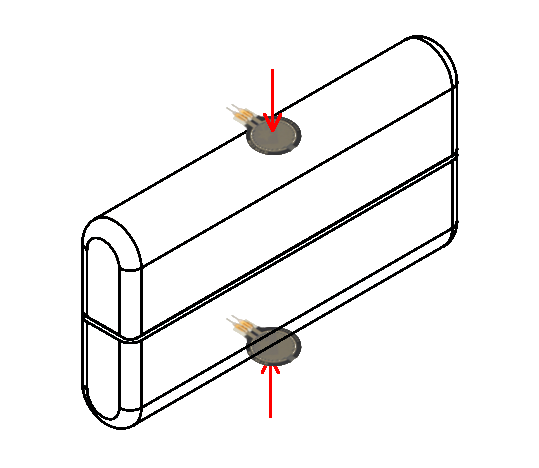
\includegraphics[width=\textwidth]{Figure/dummipalmfsr.png}
    \caption{Sensorized palm with FSR sensors}
    \label{fig:dummifsr}
  \end{minipage}
  %\caption{FSR sensors position on sensorized palm}
\end{figure}



The experiment is executed with a participant applying different forces on the above mentioned device, and recording the output from the FSR sensors and from the load cell of the \textit{sensorized palm}.
The plot in Fig. \ref{Fig:FSRcalibratedModel}, shows the data obtain from this experiment.
A toolbox for data fitting from Matlab has been used in order to find the best linear fitting equation, according to the Least Mean Square Error to the raw data, which analytically is:\\
\begin{equation}
y = 135.8 x + 1336
\end{equation}
where $y$ is the value taken as the sum of the FSRs sensors, in this experiment two FSRs has been used.
The variable $x$ is the value from the \textit{sensorized palm}, returning Newtons, used to find the best first order model to map the FSRs values.\\

 
\begin{figure}[ht]
\centering
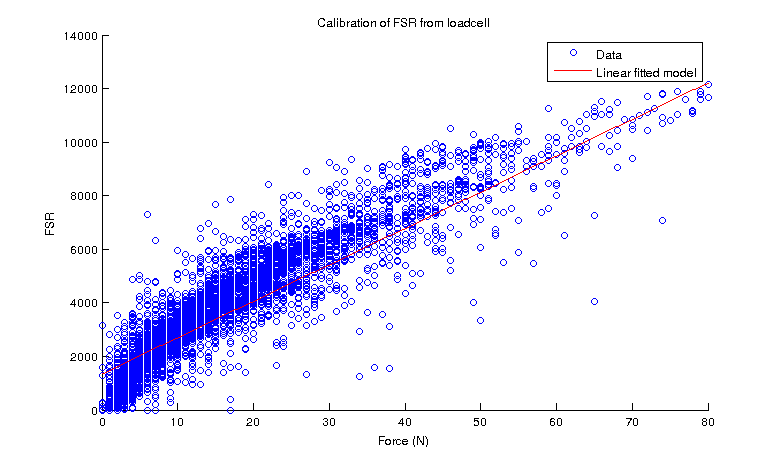
\includegraphics[width=\textwidth]{Figure/dummytofsr.png}
\caption{FSRs vs. Load Cell data}
\label{Fig:FSRcalibratedModel}
\end{figure}

Obviously, more advanced models can be fitted in order to have FSR sensors returning Newtons with a higher precision, but for the specific task required in this work is not necessary to increase the degree of the model. The handshake event is involving grasping forces in the range of the above-mentioned calibration so the force-plots in the next chapters will be intended to be Newton scaled.

\chapter{Software setup}
The described experiments can be implemented using a software capable of exchanging informations between robots, without the interaction of a human. A tool named Robot Operative System has been chosen in order to manage the informations between the devices involved in these experiments.  
\section{Ros}
The Robot Operative System (ROS) is a set of frameworks and libraries useful for robot software development. The logic of this software is really intuitive, it lets the developers to represent a device as node inside a graph. The most important node is this graph is the \textit{Master}, which is managing all the messages in the system. Each node in order to send or receive messages to/from other nodes must communicate this intention to the \textit{Master} node, which is processing the request and forwarding the right informations.\\
The ROS graph is done using a network of process called ROS nodes.
The main concepts in the ROS graph are ROS Nodes, Master, Parameter server, Messages,
Topics, Services, and Bags. Each concept in the graph is contributed to this graph
in different ways.
Each message in ROS is transported using named buses called topics. When a node sends a message through a topic, then we can say the node is publishing a topic. When a node receives a message through a topic,
then we can say that the node is subscribing to a topic but the production of information and consumption of it are decoupled. Each topic has a unique name, and any node can access this topic and send data through it as long as they have the right message type. The type of a message can be chosen among the standard primitive types (integer, floating point, Boolean, and so on) or we can define custom message types.
%The ROS graph is oriented since the messages between nodes are edges of the graph passing the information from the node who is publishing to the one subscribed to it.

\section{Nodes}
The main aim of ROS nodes is to build simple processes, this makes debug easier and simplify the structure of a project. Each ROS node is written using ROS client libraries such as roscpp and rospy, in short a ROS node can be written as a C++ source file or as a python executable program. \\
\subsection{Pisa/IIT SoftHand node}
Pisa/ITT SoftHand is provided with a variety of ROS packages, in particular, ROS node \textit{qb\textunderscore force\textunderscore interface} is the node managing the proportional controller on the position of the Pisa/IIT SoftHand. This node is publishing a topic named: /qb\textunderscore class/hand\textunderscore measurement which embeds a custom field structure named: qb\textunderscore interface/handPos. Custom field structure of messages are useful in order to send different message type over the same channel (topic).\\

\subsection{FSRs node}
The FSRs are connected to a bare PCB, each one following the circuit diagram in Fig. \ref{Fig:FSRcircuit}; This allows the source code flashed on the Arduino to: read the voltage difference at FSRs terminals, apply the linear model for force measurements and publish the information to ROS. A specific protocol called \textit{rosserial} is used in order to implement a ROS node with Arduino Uno.\\

\subsection{Auxiliary nodes}
The hardware nodes of the project are now up and running, but in order to manage the informations and to eventually save files during the execution of the experiments, auxiliary nodes are created.
The auxiliary nodes are written in C++ or Python and the choice is strictly related to the compatibility with specific library (f.i. \textit{SMACH} State MACHine is a library used to implement state machines, currently only available in Python).
Several auxiliary nodes have been created in order to manage:
\begin{enumerate}
\item FSR calibration experiments
\item Saving data during experiments
\item Open loop experiments
\item Closed loop experiments
\end{enumerate}
Again, ROS provide the concept of node which is extremely useful for splitting work in smaller and more manageable units.\\

\chapter{Open Loop Experiments}
The open loop experiments aim to verify the hypothesis that the human response to a robot handshake can be modelled as a dynamical model. In these experiments human participants are intended to be a natural calibration system for the robot grasping force $F_r$. Participants are asked to apply the force that they are perceiving during the experiments.
The force is exchanged during a handshake only after the reference position has reach the first contact point $q_0$, therefore for values of $q < q_0$ no force will be exchanged in the handshake.\\
\begin{equation}
F_{r}(q)=\left\{\begin{matrix}
k_{r}(q-q_0) & $ for $ &q-q_0 \geq 0 \\ 
0 & $ for $ & q-q_0 < 0
\end{matrix}\right.
\label{EQ:genericForce}
\end{equation}\\
%
%$$
%F_{r} = 
%  \begin{cases} 
%    $Dynamic to find$ & q-q_0 \geq 0 \\
%    0 & q-q_{0} < 0
%  \end{cases}
%$$\\

Where $F_r$ is the force during the handshake applied by the robot on the participant's hand, $q$ is the reference position sent to the device.
During these experiment each reference position of the Pisa/IIT SoftHand is held for 3 seconds, the frequency rate of is set to 100Hz. 
A file standard has been created in order to compare different experiments. The file is a '.csv' file with columns [FSR1, FSR2, FSR3, FSR4, Current, Real Position, Reference Position]. All the plots below are obtained as processing files with the previous structure. Each experiment starts with reference position set to 0 and finish with the reference position set to 0. 
The experiments are in open loop so in order to avoid injuries an emergency function has been created, if the participant starts feeling pain the key 'x' on the keyboard must be pressed. The Pisa/IIT SoftHand will take as reference position 0 (fully open) and the whole program will be stopped.
In case of emergency the file will be saved and the last data can be used to understand the configuration just before the trigger event.\\
The experiments are done with the Pisa/IIT SoftHand in a horizontal position (palm facing down) Fig. \ref{Fig:palmdown}. In this way the weight of the Pisa/IIT SoftHand will not affect the FSR readings. \\

\begin{figure}[ht]
\centering
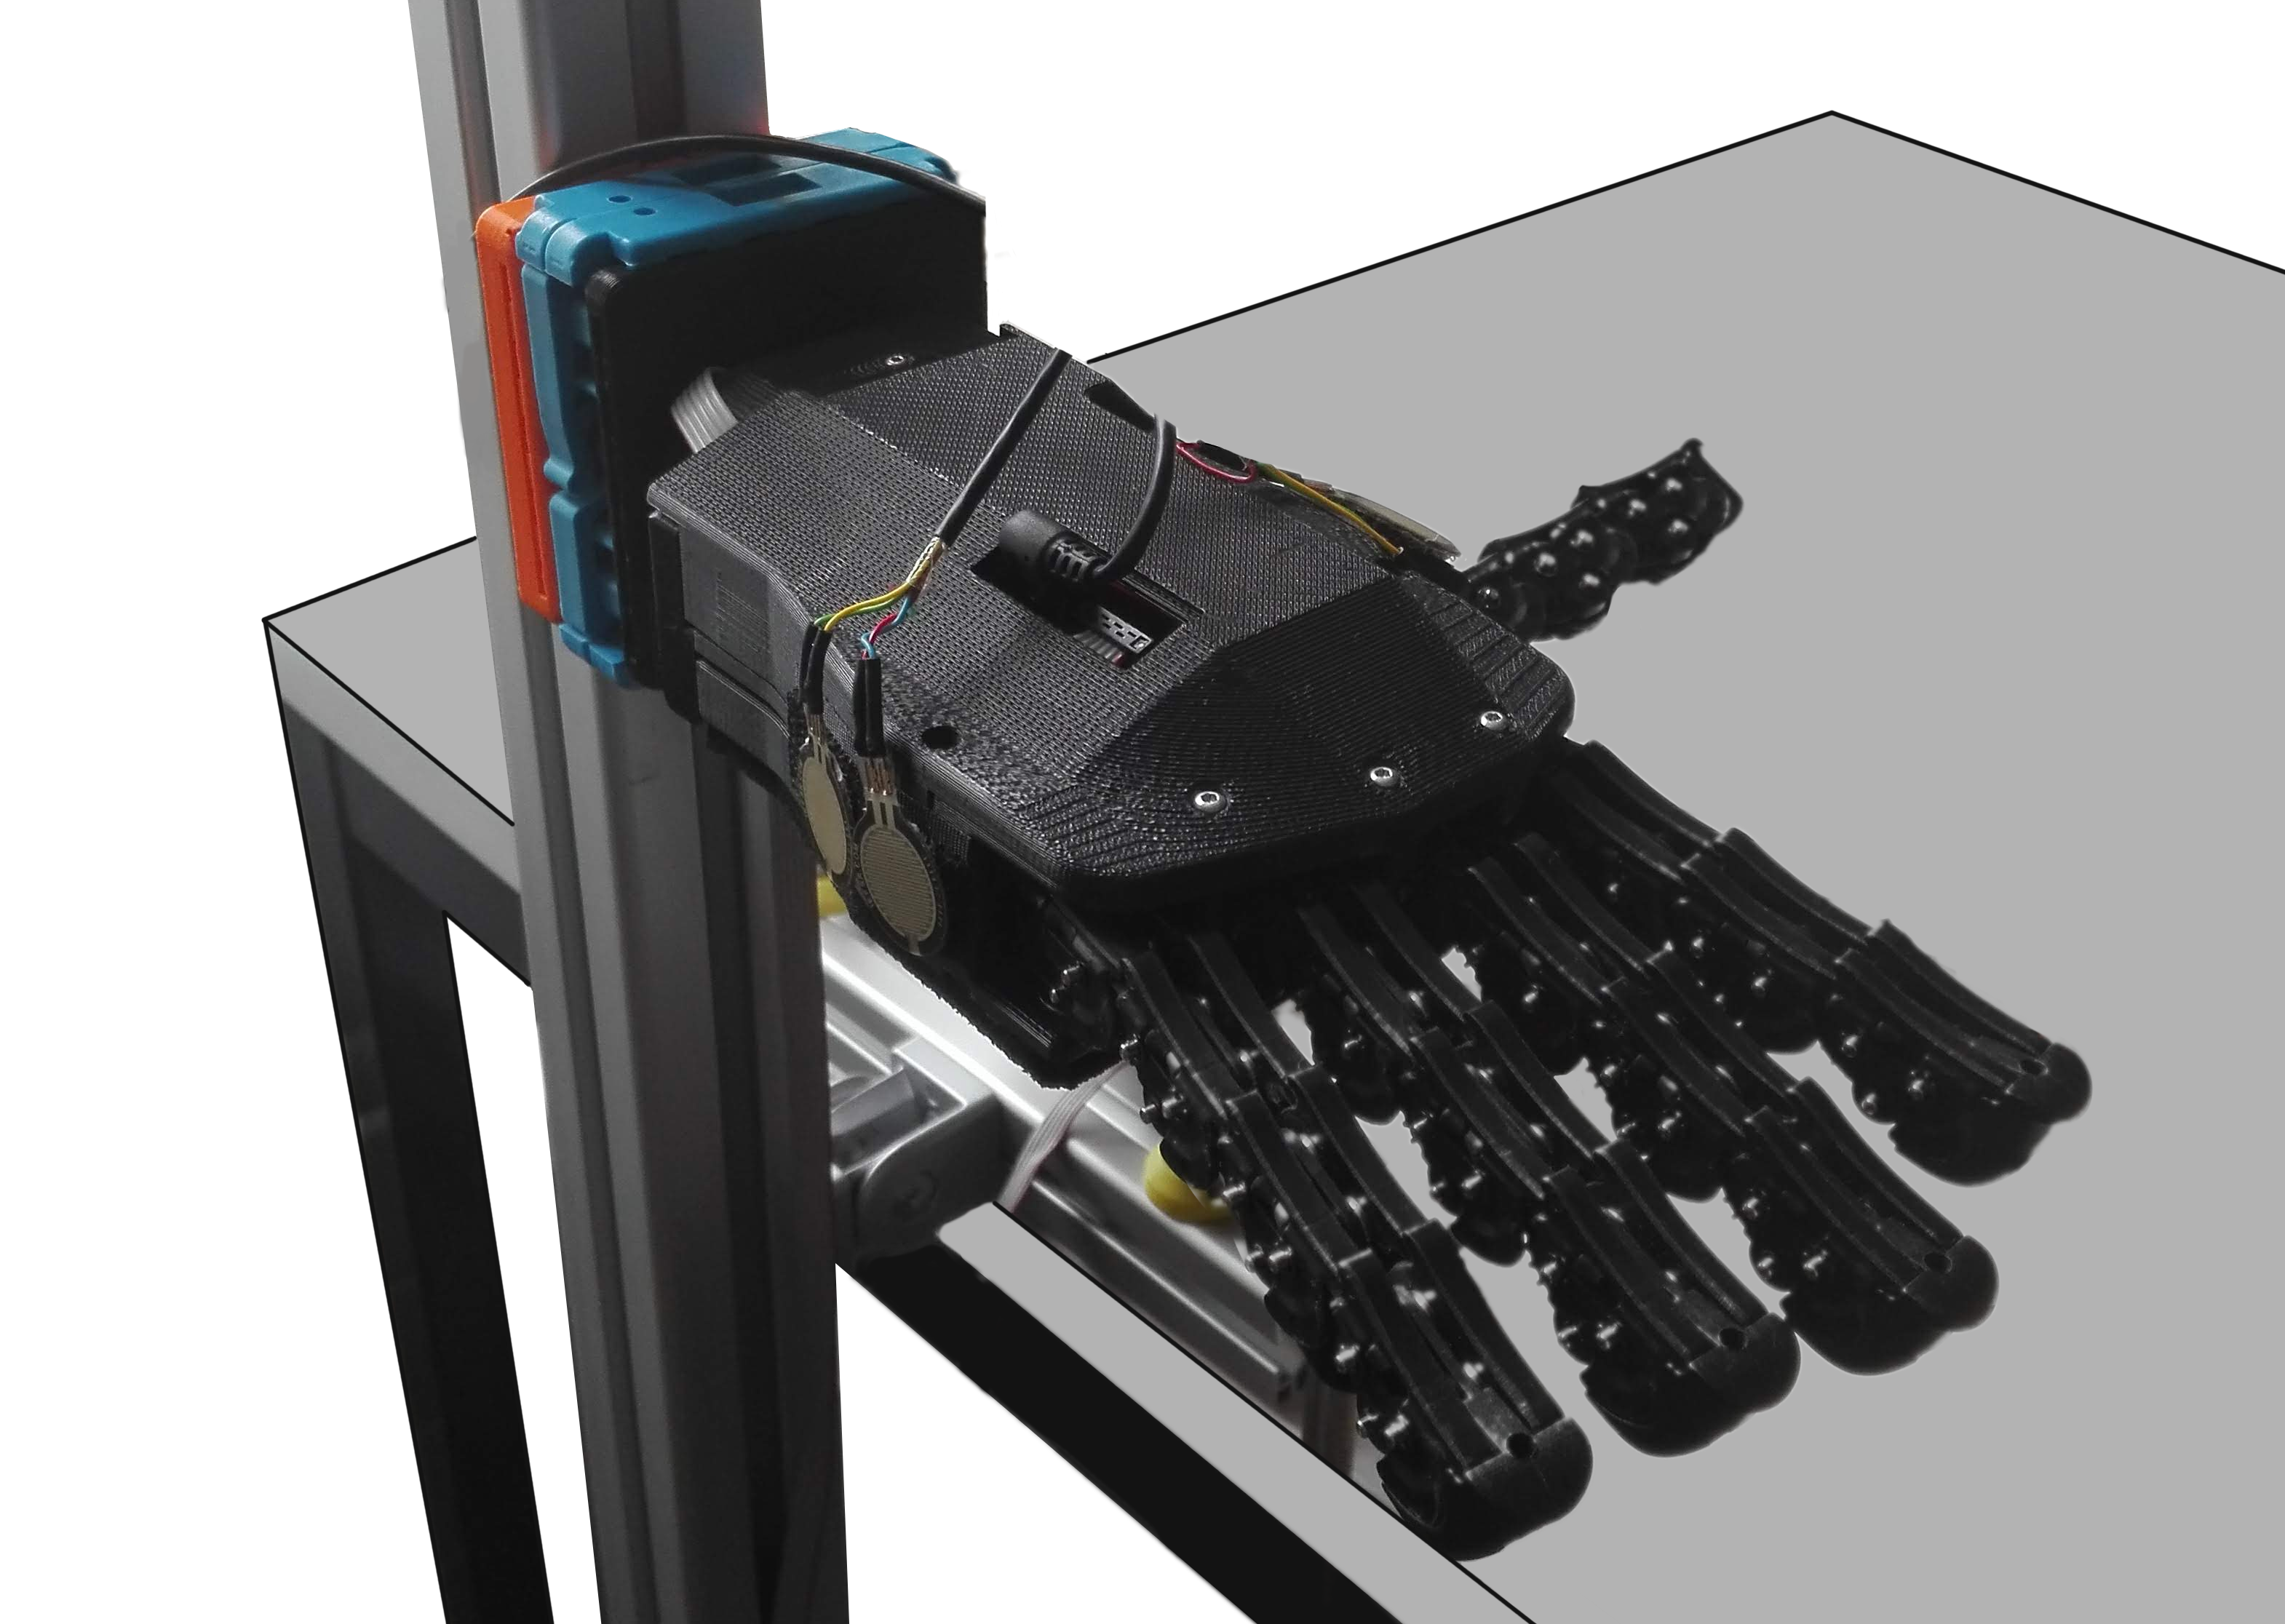
\includegraphics[width=0.6\textwidth]{Figure/stand.png}
\caption{Palm facing down environment}
\label{Fig:palmdown}
\end{figure}
\newpage
\section{Step input}
The simplest signal that can be sent to the Pisa/IIT SoftHand is a step signal on the reference position, in this way the participant's response can be evaluated. The step signal in this experiment is formally a shifted and scaled step signal, the transformation parameters has been chosen in order to start from a position without physical contact ($k_0 = 8000 $) to a position where empirical experiments have shown a consistent contact ($k_1 = 15000$). The first three seconds of the experiment $k_0$ is sent, then $k_1$ is sent so that the whole experiment lasts 6 seconds.\\
\begin{equation}
Q_{r}(t)=\left\{\begin{matrix}
k_{0} & $ for $ & t < t_0 \\ 
k_{1} & $ for $ & t \geq t_0
\end{matrix}\right.
\label{EQ:StepSignal}
\end{equation}
%$$
%Q_r(t) =   
%\begin{cases} 
%k_0 & t < t_0\\
%k_1 & t \geq t_0
%\end{cases}
%$$
%with $k \in \mathbb{R}$.

A correlation between the reference position of the Pisa/IIT SoftHand and the values recorded from the FSRs is expected. The participants are naturally applying a force ($F_{h}$) which is supposed to be proportional to the one applied from the robot to their hand during the handshake.
The same experiment has been executed with multiple participants, in order to increase the amount of data available for the model estimation. The values of reference position in this experiment are not changing during multiple trials, therefore the participants were able to predict that at $t=t_0$ a higher reference signal was sent. This behaviour has been considered not consistent to apply in post processing a model fitting of the data. 

\section{Pseudorandom input}

\chapter{Closed Loop controllers}
\section{Empirical Proportional controller}
\section{Human-calibrated controller}
\chapter{Results}

\chapter*{Conclusion}
This project applies learning \cite{art:rif.1} techniques to MNIST handwritten dataset. As we can see in the previous confusion matrix the accuracy of the final work is $97.6\%$. The overall idea is to train \emph{autoenc1},  \emph{autoenc2} and \emph{softmax1} once per time and to crop the nets in order to have coherents dimension between network interconnections. At the end of \cite{book:rif.2}this process we stack all the partial neural network together and the deep neural network come to life. \\The satisfaction behind this project can be experimented by running the file "MNIST\textunderscore drawsim.m" which is a matlab function that allows the user to draw a digit and returns the correct digit value 97,6 times over 100.